\documentclass[UTF8]{ctexart}
%字体配置
%\documentclass[UTF8]{ctexreport}
%以上是报告版,可以添加章节
%这里可以书写注释
\usepackage{graphicx}
\usepackage{caption2}
\usepackage{subfigure}
\usepackage{float}
%以上是使用图形包(傻瓜加入完事了)

\title{人机工学:个人调查报告}
\author{陈禹汀}
\date{2020/10/3}
%以上为文章属性设置

\begin{document}

\maketitle%自动制作标题

\tableofcontents%生成目录

%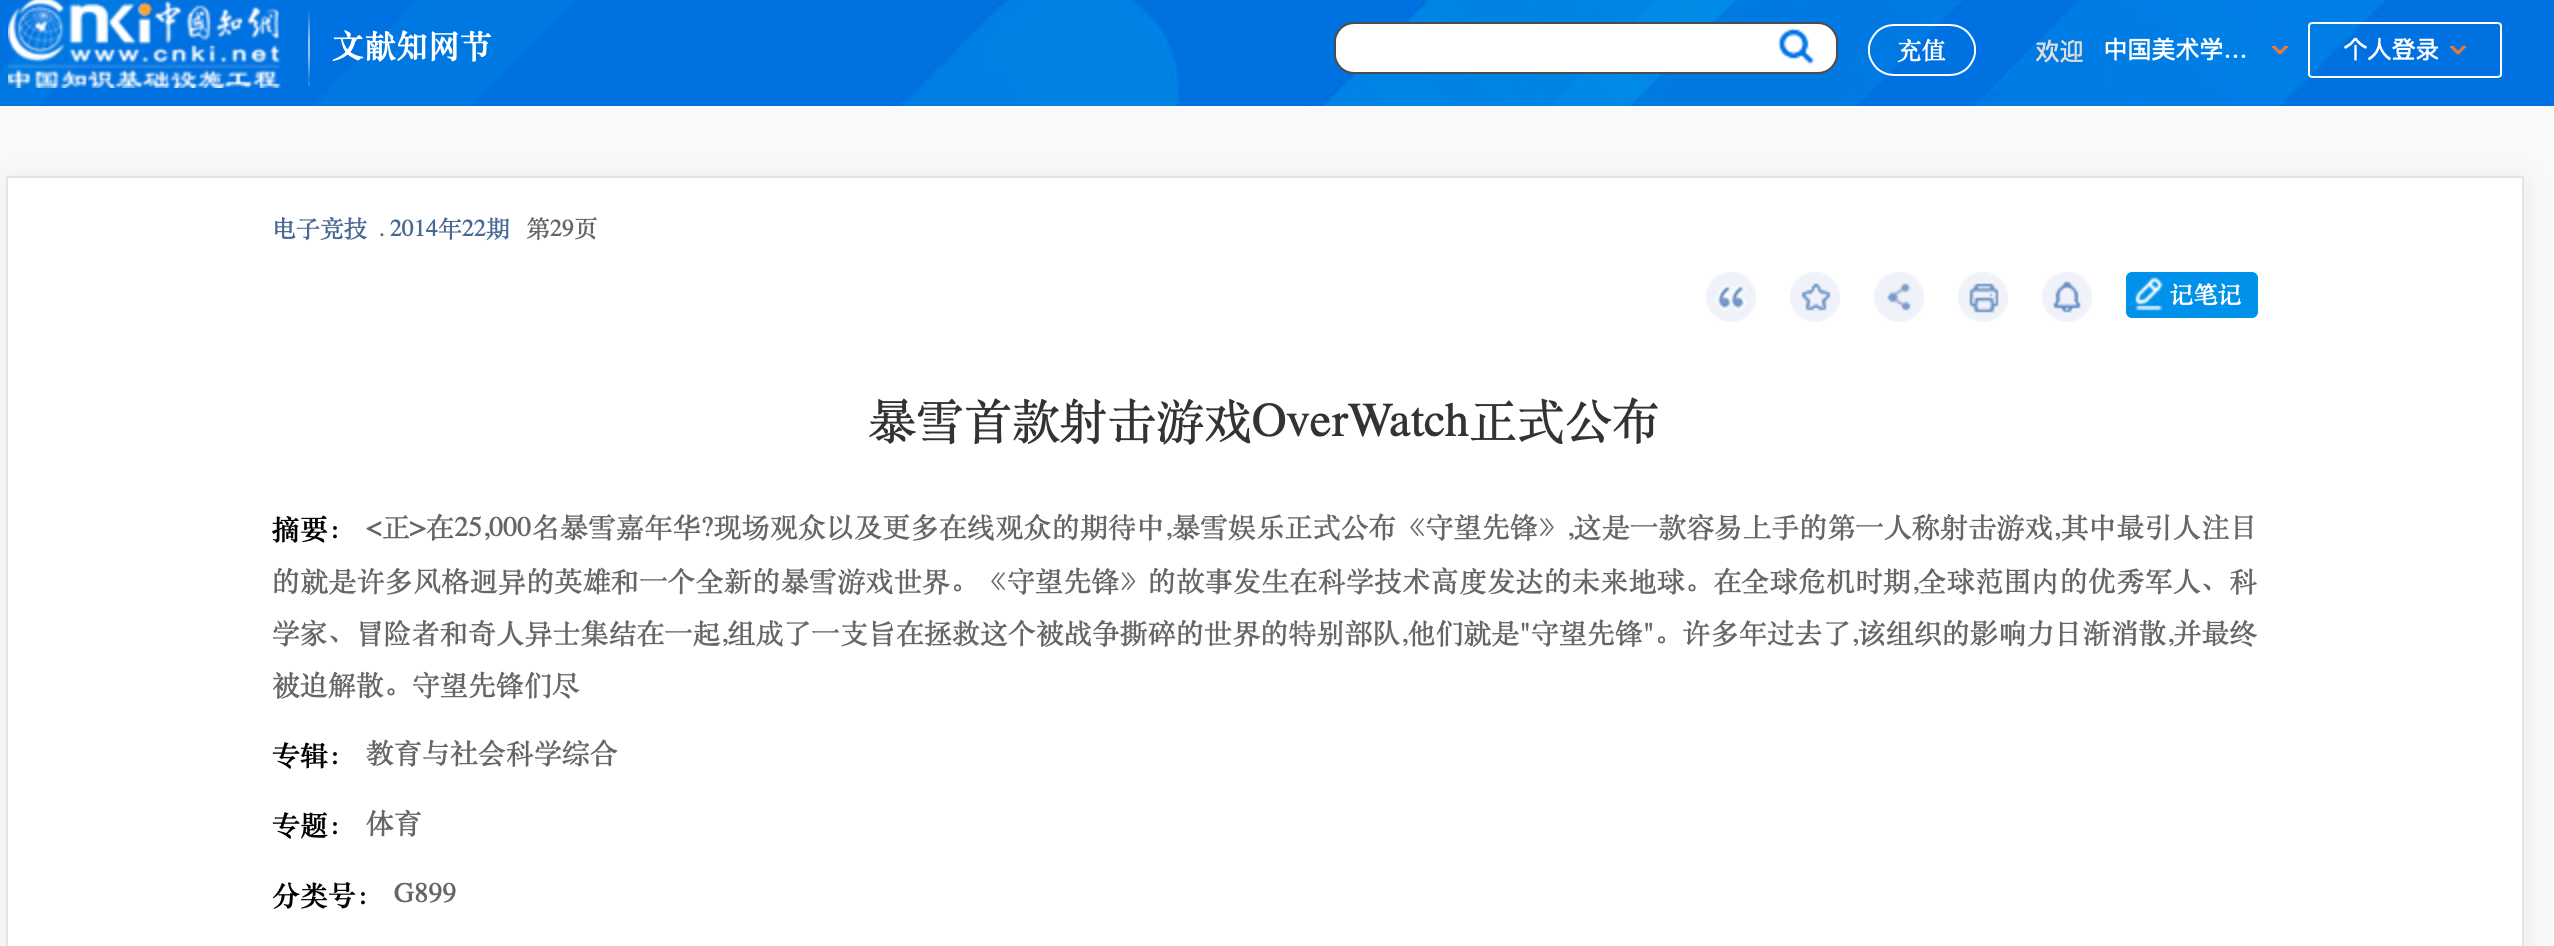
\includegraphics[width = .8\textwidth]{1.png}
%以上是插入图片
\section{china!}
    建 国 大 业
\subsection{trump}
    “真的假的。他感染了Covid-19??“
\paragraph{川建国}
    这是中国的伟大工程,他在国庆为祖国献礼,夺冠的事迹传满华夏大地。这样一种奉献精神,是切实为中华人民共和国着想。

    这是非常难得的行为,他 "Make America Great Again", 极大调动了华夏人民的劳动生产积极性。促进了中国的生产内力增长。
\paragraph{他改变了美国}
    他真的是太厉害了,他成功地使美国的中产人群对社会有了充分的认识,打破了他们社会稳定的幻想,增加了他们对共产主义对信仰。

    这是非常勇敢的行为,建国顶着重重社会压力和刻板印象,成功地使黑人群体显现了他们的本质,成功地在物理上消灭了贫困人口,而这些对于PRC的统一大业都是不可忽视的阻碍。
\subsection{him}
    he is a time traveler. he talks and laughs like the sound of the wind with a reporter named Walles. he defined the speed of HongKong news reporter. he is the one represented "not naive".
\end{document}